% !Mode:: "TeX:UTF-8" 

\BiChapter{基于聚类的克隆代码演化特征分析}
{An Analysis for Code Clone Evolutionary Characteristic Based on Clustering}

%%\BiSection{引言}{Introduction}
\BiSection{摘要}{Abstract}
软件系统中存在大量的克隆代码,克隆代码是软件中存在的彼此相似的代码片段。随着软件的演化,克隆代码也会随之发生变化,我们称之为克隆演化。在大量克隆代码及其演化过程中,必然存在着一些隐含的信息,称之为克隆演化特征,克隆演化特征可以帮助维护人员理解和维护克隆代码。遗憾的是,当前研究中对克隆演化特征的研究依然较少。为了分析并获得克隆演化特征,本文从三个方面对克隆代码及其演化过程进行分析:克隆片段、克隆组和克隆家系。通过提取不同的度量值分别表示克隆片段、克隆组和克隆家系,并在此基础上使用聚类分析的方法提取克隆代码的演化特征。在两个开源系统上进行了实验,实验结果表明,在演化过程中大部分的克隆代码是较为稳定的,有一部分克隆代码甚至是极端稳定而从未发生变化。于此同时,也存在一定数量的发生变化的克隆代码,在这部分发生变化的克隆代码中发生一致性变化的克隆代码要多于不一致变化的克隆代码。因此, 本文建议开发人员应该更加关注寿命比较长的克隆代码,同时当克隆代码发生变化时应考虑该变化是否满足一致性变化。

%%\BiSection{克隆代码演化及其相关研究}{Code Clone Evolution and its related work}
\BiSection{引言}{Introduction}
克隆代码是根据某种相似性定义彼此相似的代码片段的集合\cite{roy2007survey}。它们在软件系统中比例占到7\%~23\%,甚至在某些软件中达到59\%\cite{koschke2007survey}。由于克隆代码会随着软件系统演化,Kim等人提出了克隆家系描述克隆代码的演化过程,并且同时定义了几种克隆演化模式描述克隆代码在两个相邻版本之间的变化和不同\cite{kim2005empirical},这也引发了研究人员对克隆演化及其克隆演化模式的研究热潮。目前,研究人员开发出了大量的克隆检测工具和克隆家系的构建工具。这些工作也导致了大量的克隆分析工作,尤其是克隆稳定性研究和克隆变化研究\cite{inoue2012experience}\cite{krinke2008cloned}。

与此同时,克隆代码的有害性研究也一直是克隆研究领域争论的焦点问题。一些研究人员认为克隆代码的存在是有害的,因为它们可能会导致额外的维护代价\cite{kapser2006cloning},甚至也会导致软件缺陷,例如在演化过程中的克隆不一致变化往往会导致不一致性缺陷\cite{inoue2012experience}。因此,软件开发人员应该采取相应的措施避免克隆代码的产生,并通过重构的方法移除克隆代码。相反地,也有研究人员催克隆代码的存在持积极的态度。他们认为克隆代码是必不可少的一种软件复用方式,同时大部分产生的克隆代码比非克隆代码更加稳定,克隆复用也会节约大量的开发时间\cite{krinke2008cloned}。

无论对克隆代码采取什么样的态度,克隆代码在软件中随处可见,这是由于软件开发人员为了节约开发时间会通过粘贴复制操作引入克隆代码。因此,理解克隆代码的存在及其演化过程,并分析克隆代码对软件开发和维护过程产生什么样的影响是十分必要的。例如分析结果可以实质地帮助克隆维护和管理过程,还可以从演化的角度提供一些全新的建议和理解。自始至终,本文使用克隆演化特征描述克隆代码在演化过程中所表现出来的特征。

本文基于机器学习方法提出了一种探索和分析克隆演化特征的方法。通过映射相邻版本的克隆代码构建系统的克隆家系。然后,提取相应的度量值从三个不同的角度表示不同的克隆实体:克隆片段、克隆组和克隆家系。这些度量值涵盖了许多我们感兴趣和有价值的克隆信息。最后,我们使用WEKA( “Waikato Environment for Knowledge Analysis” \cite{hall2009weka})中实现的X-means\cite{pelleg2000x}方法聚类所有的克隆代码,并在两个软件系统上进行了实证研究。我们的实证研究的实验结果表明:一般来说克隆代在其演化过程中是较为稳定的,在其演化的初始阶段不容易发生变化。程序开打人员因此应该需要更多的关注那些在系统中存在了一定时间的克隆代码(寿命较长的克隆代码)。
同时,当克隆代码发生变化的时候,我们也建议尽可能的考虑一致性变化。
本文的创新点如下:
\begin{itemize}
\item 本文提出了一个框架分析克隆代码的演化特征,可以帮助程序维护人员维护和管理克隆代码。
\item 本文从三个不同的角度视为将克隆代码一种数据进行分析:克隆片段、克隆组和克隆家系,并提取了相应的度量值表示克隆代码。
\item 本文在两个开源系统上进行了实证研究并获得了相关的克隆演化特征,可以帮助理解和维护克隆代码。
\end{itemize}

\BiSection{相关工作}{Related Work}
克隆代码研究领域中最活跃的研究分支是克隆检测。在过去的20年中,研究人员提出了许多种克隆代码检测方法,并开发了大量的克隆检测工具,例如NiCad\cite{roy2008nicad}、CCFinder\cite{kamiya2002ccfinder}等。有兴趣的读者可以参考文献\cite{rattan2013software},该文献从不同的角度评价了不同克隆检测工具和方法。
然而,克隆检测并不能完全解决克隆代码所引发的维护困难的问题。因此,克隆管理进入了研究人员的视野,并成为克隆研究领域的新的研究热点\cite{roy2014vision}、\cite{koschke2012software}。JSync是一个克隆管理工具,可以帮助管理系统中的克隆代码并维护其一致性\cite{nguyen2012clone}。同时,CloneTracker是一个eclipse插件,可以帮助软件维护人员跟踪系统中的克隆代码\cite{duala2008clonetracker}。而工具CeDAR将克隆重构集成到软件开发环境中,从而方便的对克隆代码进行重构\cite{tairas2010representation}。

同时,克隆代码分析也是克隆代码领域的另一个重要研究内容,可以有效的帮助程序开发人员理解克隆代码以及对系统的影响。Yang等人提出了一个分类模型可以帮助评价克隆代码\cite{yang2015classification}。Qu等人提出了一个模式挖掘的框架可以分析系统中的克隆代码情况\cite{qu2014pattern}。Lin则提出了一个克隆代码差异性分析的方法用于帮助克隆代码分析,可用于克隆重构中\cite{lin2014detecting}。

克隆代码一直随着软件系统演化,研究人员一直对克隆演化过程以及克隆演化特征有着极大的研究兴趣。Kim提出了克隆家系的概念用于描述克隆代码的演化过程,并使用演化模式帮助理解克隆代码在演化过程中的变化情况,并且还注意到克隆重构可能并不能提高软件质量,因为以下原因:克隆可能是短寿命的,或者长期存在的克隆一致地改变通常不容易重构\cite{kim2005empirical}。Duala-Ekoko提出了一个克隆追踪系统,使用CRD描述克隆代码的上下文信息并以此追踪克隆代码的变化,并及时通知程序开发人员\cite{duala2010clone}。Bakota提出了一种将克隆代码从一个特定版本的映射到另一个版本的方法,并提出克隆气味的定义帮助开发人员确定与软件缺陷相关的克隆\cite{bakota2011tracking,bakota2007clone}。 Krinke发现克隆代码比非克隆代码更加稳定,并且平均寿命也比非克隆代码长\cite{krinke2008cloned}。 Bettenburg观察到所有克隆家系中只有1.02\% ~ 4.00\%的克隆代码会引入软件缺陷,因此克隆代码对软件的质量并没有显著影响\cite{bettenburg2009empirical}。  Harder发现克隆代码的稳定性主要取决于克隆代码对应的具体软件项目的特性\cite{harder2013cloned}。

同时,有关克隆代码有害性的讨论一直是克隆领域持续争论的热点问题。克隆代码是有害的这种观点的支持者认为克隆代码的存在可能导致额外的维护工作,而软件演化过程中的克隆不一致地改变更可能导致软件缺陷\cite{inoue2012experience}。持反对意见的研究人员认为克隆代码在软件演化过程中通常比非克隆代码更加稳定\cite{krinke2008cloned}。 Foyzur Ra​​hman通过分析克隆和缺陷之间的关系发现:首先,大多数缺陷与克隆代码无明显的相关性。其次,克隆代码比非克隆代码具有更少的缺陷\cite{rahman2012clones}。
 于此同时,还有一些研究人员对克隆代码是否有害持中立态度。  Cory Kapser描述了克隆代码的几种模式,并讨论了不同克隆模式的优缺点,研究发现有的模式显示克隆代码是有益的,有的则显示克隆代码是有害的\cite{kapser2006cloning}。  一些研究人员使用贝叶斯网络,一种机器学习技术,预测克隆代码的有害性\cite{wang2012can}。  我们认为,并且如本研究中的发现所显示的,克隆的存在是开发者在软件开发期间所采用的习惯的性质,并且对进化过程中克隆的变化的一致性的注意可以在缓解软件维护努力。

\BiSection{基于聚类的克隆演化特征提取方法}{The Approach for Clone Characteristic Analysis based on Clustering Methold}
\BiSubsection{克隆演化特征分析框架}{ The Framework of Clone Characteristic Analysis}

见图~\ref{framework2}是本文的基于机器学习的克隆代码演化特征分析框架。可将其划分为:预处理、度量提取和特征分析三个阶段。 在预处理阶段,本文通过映射连续软件版本的克隆代码以及克隆组来构建相应的克隆家系。 在度量提取阶段,我们分别识别和提取相应的度量,用于分别表示克隆片段、克隆组和克隆家系。这些度量值提取了捕获克隆代码及其进化的相关信息。 最后,在特征分析阶段,我们使用机器学习技术(聚类方法)来探索克隆代码的克隆演化特征。

\begin{figure}[htbp]
\centering
\includegraphics [width=0.4 \textwidth ]{Fig2-1.pdf}
\bicaption [framework2]{}{基于聚类的克隆演化特征提取方法框架}{Fig.$\!$}
{The Framework of Clone Characteristic Analysis}\vspace{-1em}
\end{figure}

\BiSubsection{预处理阶段}{ Pre-processing}
在这个阶段,我们的目标是根据克隆检测工具所检测的连续版本软件中的克隆代码构建克隆系谱。我们首先获得连续版本的开源软件,主要来源于网站和版本控制系统,并用NiCad检测每个软件版本中的所有克隆代码。NiCad会根据克隆代码的相似性将所有的克隆代码划分为克隆组。之后,我们使用CRD描述克隆代码,并通过关联相邻的克隆片段和克隆组来构建克隆系谱。

{\em 使用NiCad进行克隆检测和使用CRD(克隆区域描述符)进行克隆表示}。 NiCad是一个克隆检测工具,它可以有效地发现系统中克隆代码。我们使用默认配置来检测每个软件版本的所有克隆代码,检测工具有两个不同粒度的克隆代码:函数克隆和块克隆。因为{\em 块级别}更通用(函数克隆也是是块克隆代码),我们使用{\em 块级别}的默认配置来检测每个软件版本的所有克隆代码。克隆检测结果保存在XML文件中,这些文件用{\ em``Filename + Line No''}标记克隆片段。同一组内的克隆代码彼此之间是相似的。为了构建克隆家系,我们使用修改后的CRD的来描述克隆代码,原CRD这是由Duala-Ekoko提出。CRD是克隆代码的抽象描述,包括文件名、方法名、并结合句法,结构和词法信息等\cite{duala2010clone}。 我们结合CRD中的{\em LocationOverlapping}和{\em TextSimilarity}来来映射两个相邻版本中的克隆代码和克隆组。{\em LocationOverlapping}可以帮助找到源代码中的克隆片段\cite{kim2005empirical},并计算版本$ i $和版本$ i + 1 $中克隆片段位置之间的重叠分数。{\em TextSimilarity}可以用于比较克隆片段的相似性,这里使用NiCad\cite{roy2008nicad}中的计算方法。它计算两个克隆片段的常用代码行的百分比。%%添加详细的算法描述。

{\ em映射克隆组以及构建克隆家系}。为了构建克隆系谱,我们将两个连续版本之间所有的克隆片段和克隆组进行映射,映射算法称为基于CRD的克隆组映射算法。给定两个相邻的软件版本{\em $v_i$}和{\em $v_ i + 1$},我们比较{\em $v_i$}中的每个克隆片段与每个克隆片段并且产生成对的映射克隆片段,使得对于每对,(1)第一克隆片段来自{\em $ v_i $},而第二个克隆片段来自{\em $ v_ {i + 1}$ },和(2)克隆组也可以用匹配的克隆片段进行映射。 
%%算法的细节在我们前面的工作[25]中描述。
接下来,我们可以基于映射克隆组为软件构建克隆家系。克隆组映射后,我们可以使用演化模式描述克隆组在其进化过程中的变化,即{\em ``clone pattern''}。更正式地,每个克隆组(称为Clone Group,简写为CG)可以包含几个克隆片段(称为Clone Fragment,CF)。我们假设存在于两个相邻版本中的一个克隆组,使用{\em srcCG}表示前一版本中的克隆组,{\em destCG}表示后一版本中的克隆组,从{\em srcCG}到{\em destCG}的变化更改由克隆模式描述,并且它们成为与{\em destCG}关联的度量。

克隆模式由Kim 定义,给出如下:
\begin{itemize}
\item {Static模式}: no change in clone fragment  (number and content).
\item {Same模式}: no change in number of clone fragment, but the  content of fragment may change.
\item {Add模式}: number of clone fragment increases.
\item {Subtract模式}: number of clone fragment decreases.
\item {Consistent Change模式}:  all clone fragments change consistently.
\item {Inconsistent Change模式}: clone fragments change inconsistently.
\item {Split模式}: inconsistent change beyond a threshold, causing the clone group to split into two clone groups.
\end{itemize}

\begin{figure}[htbp]
\centering
\includegraphics [width=0.4 \textwidth ]{Fig2-2.pdf}
\bicaption [gena1]{}{克隆家系示意图}{Fig.$\!$}
{An Example of Clone Genealogy}\vspace{-1em}
\end{figure}

图\cite{gena1}给出了克隆系谱和克隆模式的实例。 在该实施例中,从该软件的5个版本构建克隆系谱。从版本{\em i}到{\em i+1},克隆组用两个新的克隆片段扩大,因此其关联的克隆模式是{\em add}。在下一个版本更改中,克隆组分为两组,具有不同的克隆模式(一个是{\em subtract},另一个是{\em consistent change})。 从版本{\em i+2}到{\em i+ 3},克隆模式分别是{\em sub}和{\em 不一致的更改}。在最后一个版本中,克隆模式分别是{\em add}和{\em sub}。

\BiSubsection{提取阶段}{ Extracting Clone Metrics}

正如在机器学习中通常所做的那样,我们使用特征向量表示克隆代码,并将之称为{\em 克隆度量}。 这些特征分别从克隆片段、克隆组和克隆家系中进行提取。

{\em 克隆片段的度量}:克隆片段给出了克隆代码本身的一些特征。在克隆代码片段的生命期间,克隆代码片段可以由开发人员修改,特别是在软件维护期间。因此,克隆片段在演化过程中可能发生变化,也可能发生多次变化。因此,我们将克隆变化的次数和从上一版本中是否发生了视为度量。 因此,版本$ i $中克隆片段的度量标准如下:
\begin{itemize}
\item {Clone Life}: number of versions which the clone fragment exists in software so far (until version i).
\item {Ischanged}:	equals 1 if the Clone fragment in version i is changed from the last version (version i-1); 0 otherwise.
\item {Change Times}:	number of times the clone fragment changed so far (up till version i) in the evolution.  
\end{itemize}

{\em 克隆组的度量值}。克隆组提供克隆组的一些区域性特征。这里的克隆组是指在同一版本中的克隆代码所组织成的克隆组。对于在软件版本中发现的克隆组,最重要的是捕捉其寿命长度。在进化过程中,大部分的克隆组会从上一个版本演化为当前版本,仅有少部分新产生的克隆代码。为了描述这种变化,Kim将之称为{\em clone pattern},即克隆组的演化模式。演化模式可以给我们克隆组在进化过程中的变化进行总结。因此,我们将版本$ i $ 中克隆组的寿命和克隆模式提取为度量,如下所示:
\begin{itemize}
\item {Group Life}: number of versions which clone group exists in software till version $i$.
\item {Static}:	all clone fragments in group are static from last version.
\item {Same}:	clone group undergoes a ``same'' pattern change from  last version.
\item {Add}: clone group undergoes an ``add'' pattern change from last version.
\item {Subtract}: clone group undergoes a ``subtract'' pattern change from last version.
\item {Consistent Change}: clone group undergoes a ``consistent change'' pattern from last version.
\item {Inconsistent Change}: clone group undergoes an ``inconsistent change'' pattern from last version.
\item {Split}: clone group undergoes a ``split'' pattern change from last version.
\end{itemize}

{\em 克隆家系度量}。克隆家系可以提供克隆演化的全局视角,可以捕获发生在所有版本中的整个克隆进化过程的特征。一个克隆组在所有的版本中的演化情况即是一个克隆家系,因此一个软件系统中有很多个克隆家系。我们提取了{\em  克隆寿命}和{\em 克隆模式数量}来表示克隆家系。首先{\em 克隆寿命}是克隆家系的重要指标,它描述了克隆家系在系统中存在的时间。然后,克隆家系还描述了这个克隆组在整个生命中如何改变(克隆模式),从而因为这些改变可以告诉我们关于克隆家系变化的历史。因此,我们捕获克隆家系在其整个生命中经历的{\em 克隆寿命}和{\em 克隆模式的数量}。 因此,度量标准包括以下内容:
\begin{itemize}
\item Genealogy  Life: number of versions which clone genealogy exists in software.
\item Static Number: number of ``static'' pattern which all clone groups belonging to this genealogy have experienced in its life.
\item Same Number: number of ``same'' pattern which all clone groups belonging to this genealogy have experienced in its life.
\item Add Number: number of ``add'' pattern which all clone groups belonging to this genealogy have experienced  in its life.
\item Subtract Number: number of ``subtract'' pattern which all clone groups belonging to this genealogy have experienced in its life.
\item Consistent Number: number of ``consistent pattern'' which all clone groups belonging to this genealogy have experienced in its life.
\item Inconsistent Number: number of ``inconsistent pattern'' which all clone groups belonging to this clone genealogy have experienced in its life.
\item Split Number: number of ``split'' pattern which all clone groups belonging to this genealogy have experienced in its life.
\end{itemize}

\BiSubsection{克隆演化特征挖掘}{Clone Characteristics Mining}

为了从克隆代码及其进化中挖掘克隆特征,我们使用WEKA中的聚类方法来分析不同的克隆实体,分别是:克隆片、克隆组和克隆家系。我们将这个挖掘任务分成两个子任务。第一,我们对获得的每个克隆实体中的度量进行统计,并且分析这统计分析所表现出来的克隆特征。第二,我们使用WEKA对这些克隆实体进行聚类。在这个子任务中,我们的主要目标是聚类分析在软件演化过程中克隆代码的寿命以及变化的情况。具体来说,我们的目标是确定克隆变化在克隆演化中所发生的时间以及变化。为此,我们在WEKA中使用工具来对包含时间元素的克隆实体进行聚类。在这个子任务中,使用WEKA完成此任务也涉及两个部分:首先,我们为每一个克隆实体生成一个“克隆演化向量”,其中包含每个克隆实体的所有度量(包括时间度量)。第二,我们使用WEKA聚类这些向量,并从聚类获得的结果中分析并获取克隆演化特征。让我们进一步对其进行阐述。

 {\em 生成克隆载体}。 对于每个克隆片段、克隆组和克隆家系,其特征向量是一个$ m $维向量:{$ V $ = {($ v_1 $,$ v_2 $,$ ... $,$ v_m $)}},其中$ v_i $表示前一小节中提到的特定度量。当我们为所有克隆生成向量时,我们获得所有克隆的聚类向量空间X,其可以由{$ X $ = {($ x_1 $,$ x_2 $,$ ... $,$ x_n $)}定义},其中$ n $是克隆实体的数量。因为我们从三个角度考虑克隆:克隆片段,克隆组和克隆家系。因此,我们也有三个克隆载体的所有,表明三个不同的水平。以克隆组为例,一个克隆组产生一个8维向量{$ V $ =($ v_1 $,$ v_2 $,$ ... $,$ v_8 $)},其中$ v_i $(对于所有1 $ \ le $$ i $$ \ leq $ 8)是此克隆组所提取的度量值。
  
 {\em 使用WEKA聚类克隆特征向量}。WEKA是一种用于数据挖掘的机器学习工具。我们将克隆作为数据并产生相应的实体而不是克隆代码,然后使用WEKA分析所有载体(所有克隆)以获得克隆特征。 WEKA中实现了许多方法来分析数据,例如聚类,分类,关联规则等。我们对矢量空间X上的克隆片段,克隆组和克隆家系使用{\em X-means Clustering}算法。 {\ em X-means clustering}是{\ em k-means}的变体;后者旨在将$ n $向量分割为先前指定的$ k $数量的簇,使得每个向量属于其平均值最接近该向量的簇。假如使用{\ em K-means},我们需要确定聚类之前的数量。然而,对于克隆分析的情况,难以确定所需的簇的数目。因此,我们使用{\ em X-means clustering}。

X-means聚类是一种高效的算法,可以自动的搜索聚类位置的空间和优化贝叶斯信息准则度量所需的聚类数量[26],它可以自动确定集群的数量。给定一组向量(克隆)$ X $ = {($ x_1 $,$ x_2 $,$ ... $,$ x_n $)},其中每个$ x_i $是$ d $维实向量)。X-means聚类旨在将这些$ n $向量划分为$ k $ clusters $ C $ = {($ C_1 $,$ C_2 $,$ ... $,$ C_k $)},以便最小化群内平方和(WCSS)(聚类中每个点的距离函数与K中心的距离函数的和),集群中每个点的距离函数与其集群中心的总和)。我们只指定$ K $的范围值。 {\ em X-means clustering}可以有效地从范围中搜索最好的$ K $。它从给定的$ K $范围的最低值开始,并继续增加此值,直到范围的上限。在此过程中,X-means聚类使用模型选择标准计算每个$ K $的分数。它选择$ K $的最高分数输出。对于每个$ K $,x-means聚类使用迭代细化技术。首先,它将每个向量分配给其平均值产生集群内最小平方和(WCSS)的集群。第二,它计算新的均值为新聚类中的向量的质心。当分配不再改变时,算法收敛。它使用后验概率用贝叶斯信息准则对这$ j $进行评分。。

\BiSection{实验设置}{Case Study}

在本节中,我们将给出我们的案例研究。首先,我们简要描述了所使用的开源软件系统,并描述了从三个不同的克隆代码视角探索克隆演化特征的实验步骤。我们选择两个开源软件作为我们的实验系统:分别为{\em ArgoUML}和{\em jEdit}。它们都是使用Java语言开发的软件,并且它们都经历了超过10个版本的演化。{\em ArgoUML}是一个领先的开源UML建模工具,包括对所有标准UML 1.4图的支持。{\em jEdit}是另一个开源项目,是程序员开发所使用的编辑器,其特点是具有易于使用的接口,类似于许多流行的文本编辑器。\\

表~\ref{statisticsofcluster}描述了这两个实验系统的基本信息情况。具体来说,我们分别考虑$ 14 $和$ 22 $版本。对于每个软件,我们列出此实验的第一个版本(开始)和最后版本(结束)。列“克隆片段”列出从每个软件收集的克隆片段的数量(包括所有版本)。类似地,“克隆组”和“克隆家系”分别是收集的克隆组和克隆家系的数量。
\begin{table}[htbp]
\bicaption [statisticsofcluster]{}{两个开源软件实验系统信息}{Table$\!$}{The Two Open Sources Software for Experiments}
\vspace{0.5em}\centering \wuhao
\begin{tabular}{ccccccc}
\toprule [1.5pt ]
\multirow{2}{*}{Projects}&\multirow{2}{*}{Versions}&Start&End&Clone&Clone&Clone\\ 
&&Version&Version&Fragment&Group&Genealogy\\
\midrule[1pt]
ArgoUML&14&0.20.0&0.34.0&25422&7012&1036\\ 
jEdit&22&3.0.0&5.0.0&6636&2256	&237\\ 
\bottomrule [1.5pt]
\end{tabular}
\end{table}

为了探索克隆代码演化特征,我们将克隆代码分为三个不同的视角:克隆片段、克隆组和克隆家系。 首先,我们对克隆片段进行实验。 在这里,我们探讨和调查克隆片段从一个版本到另一个版本的变化情况,以及克隆片段的历史变化情况和存在系统中的时间。 其次,克隆组在软件进化过程中有一些克隆模式。 在这里,我们有兴趣确定克隆模式的类型(例如一致的变化,不一致的变化等),它们发生(或不发生)频繁(或不频繁)。最后,克隆家系实验,提供了软件的全局视图。

在每个实验中,我们使用两种方法分析克隆:第一种是使用统计方法分析克隆,第二种使用X-means聚类方法深入分析克隆。

\BiSection{实验结果和分析}{Analysis \& Results}
\BiSubsection{克隆片段实验}{Clone Fragment Experiment}

克隆片段是指软件中存在的真实的代码片段。 在其生命周期内(作为克隆),克隆片段可能会被开发人员修改,特别是在软件维护期间。为帮助分析克隆片段的变化,我们考虑克隆片段的三个度量(相对于检测到它们的软件版本):{\em clone life,ischanged and change time}。 这些将帮助我们了解克隆如何在其演化过程中的变化情况。

\begin{table}[htbp]
\bicaption[cfstaargouml]{}{ArgoUML中克隆片段的变化统计信息}{Table$\!$}{Clone Fragment  Change Statistic of ArgoUML}
\vspace{0.5em}\centering\wuhao
\begin{tabular}{ccccc}
\toprule[1.5pt]
 & \multicolumn{4}{c}{Change Times}\\
\midrule[1pt]
Change Times&0&1&2&3\\ 
Number&24327&982&109&4\\ 
Total&24327&\multicolumn{3}{c}{1095} \\
\bottomrule[1.5pt]
\end{tabular}
\end{table}

\begin{table}[htbp]
\bicaption[cfstajedit]{}{jEdit中克隆片段的变化统计信息}{Table$\!$}{Clone Fragment  Change Statistic of jEdit}
\vspace{0.5em}\centering\wuhao
\begin{tabular}{ccccccccc}
\toprule[1.5pt]
 & \multicolumn{8}{c}{Change Times}\\
\midrule[1pt]
Change Times &0&1&2&3&4&5&6&7\\ 
Number&5885&533&135&47&14&10&11&1\\ 
Total&5885&\multicolumn{7}{c}{751}   \\ 
\bottomrule[1.5pt]
\end{tabular}
\end{table}

在表~\ref{cfstaargouml}和表~\ref{cfstajedit}中,我们对克隆片段的变化进行了统计分析。从表中可以看到,大多数克隆片段在它们的演化过程中不会发生变化(在{\em ArgoUML}中为$24327$,在{\em jEdit}中为$5885$)。同时, 只有一小部分克隆片段在演化中发生了变化(在{\em ArgoUML}为$1095$,{\em jEdit}为$751$)。 还有极少数的克隆片段其生命周期中改变了不止一次。 这里,我们可以得出结论:{\em 克隆片段在其生命中非常稳定(大多数克隆片段从不改变);对于发生变化的,它们不会非常频繁地变化。}

\begin{table}[htbp]
\bicaption[cfcluargouml]{}{ArgoUML中克隆片段的聚类结果}{Table$\!$}{Clone Fragment Clustering Results of ArgoUML}
\vspace{0.5em}\centering\wuhao
\begin{tabular}{ccccccccccc}
\toprule[1.5pt]
\multirow{3}{*}{Cluster}&{Number}&\multicolumn{3}{c}{Clone Life}&\multicolumn{3}{c}{Ischanged}&\multicolumn{3}{c}{Change Times} \\
&(Percentage)&\multirow{2}{*}{Mean}& Standard &\multirow{2}{*}{Median}&\multirow{2}{*}{Mean}&Standard &\multirow{2}{*}{Median}&\multirow{2}{*}{Mean}&Standard &\multirow{2}{*}{Median}\\
&&&  Deviation&&& Deviation&&& Deviation&\\ 
\midrule[1pt]
Cluster 0&899(4\%)&7.2069&2.2993&7&0.09232&0.28965&0&1.13014&0.34963&1\\ 
Cluster 1&3082(12\%)&7.76314&1.52307&8&0&0&0	&0&0&0\\ 
Cluster 2&3006(12\%)&3.833&0.8707&4&0.05822&0.23419	&0	&0.0652&0.24692&0\\ 
Cluster 3&18435(73\%)&1.09401&0.29184	&1	&0	&0	&0	&0	&0	&0\\ 
\bottomrule[1.5pt]
\end{tabular}
\end{table}

\begin{table}[htbp]
\bicaption[cfclujedit]{}{jEdit中克隆片段的聚类结果}{Table$\!$}{Clone Fragment Clustering Results of jEdit}
\vspace{0.5em}\centering\wuhao
\begin{tabular}{ccccccccccc}
\toprule[1.5pt]
\multirow{3}{*}{Cluster}&{Number}&\multicolumn{3}{c}{Clone Life}&\multicolumn{3}{c}{Ischanged}&\multicolumn{3}{c}{Change Times} \\
&(Percentage)&\multirow{2}{*}{Mean}& Standard &\multirow{2}{*}{Median}&\multirow{2}{*}{Mean}&Standard &\multirow{2}{*}{Median}&\multirow{2}{*}{Mean}&Standard &\multirow{2}{*}{Median}\\
&&&  Deviation&&& Deviation&&& Deviation&\\ 
\midrule[1pt]
Cluster 0&	200(3\%)	&5.325	&2.6899	&5	&1	&0	&1	&1.64	&1.1476	&1\\ 
Cluster 1&	1371(21\%)	&9.07075	&2.88542	&8	&0	&0	&0	&0.50328	&0.91649	&0\\ 
Cluster 2&	1624(15\%)	&4.2266	&1.11192	&4	&0	&0	&0	&0.06466	&0.26059	&0\\ 
Cluster 3&	3441(66\%)	&1.17495	&0.37998	&1	&0	&0	&0	&0	&0	&0\\ 
\bottomrule[1.5pt]
\end{tabular}
\end{table}

在表~\ref{cfcluargouml}和~\ref{cfclujedit}是克隆片段的聚类结果。对于{\em ArgoUML}和{\em jEdit}两个开源软件中,Cluster0是所有克隆片段中数量最小的,该Cluster中的克隆代码从上一个版本演化到此版本时发生了变化,我们将此克隆称为{\em changed clone}。从表中可以看到{\em 在所有的克隆代码中很少发生变化的克隆片段,同时对于发生变化的克隆代码,发生变化的时刻往往是当它们在系统中存在一段时间后}。根据``{\em isChanged}''列,我们可以看到对于{\em  ArgoUML}中的Cluster1和3和{\em  jEdit}中的Cluster1、2和3,所有的克隆片段都没有发生变化。这意味着{\em 大多数克隆片段在其演化的过程中是稳定的}。{\em ArgoUML}和{\em jEdit}中的Cluster3是完全没有发生变化的克隆片段,根据其寿命发现它们在软件中存在的寿命极短 。这表明{\em 刚刚出现在系统中的克隆是“极其”稳定的(它们在短时间内不会发生变化)}。因此,我们应该更多地关注{\em 克隆片段存在几个版本,因为他们更容易发生变化。}

总之,只有少数的克隆代码片段在软件演化过程中会发生变化。 这些变化的克隆所经历的的变化往往通常发生在它们在系统中存在一段时间之后经历变化。

\BiSubsection{克隆组实验}{Clone Group Experiment} 

{\em clone fragment}仅仅可以提供克隆片段本身的演化属性,是一个最小的角度。而通过对{\em clone group}进行分析则提供了一个较大的角度分析克隆代码的演化情况。 %在软件演化的上下文中。每个版本的软件都有很多克隆组。
我们研究克隆组在进化过程中是如何变化的。这些更改按{\ em clone patterns}分类。

\begin{table}[htbp]
\bicaption[cgstaargouml]{}{ArgoUML中克隆组的变化统计信息}{Table$\!$}{Clone Group  Change Statistic of ArgoUML}
\vspace{0.5em}\centering\wuhao
\begin{tabular}{cccccccc}
\toprule[1.5pt]
Number of&\multirow{2}{*}{Static}&\multirow{2}{*}{Same}&\multirow{2}{*}{Add}&\multirow{2}{*}{Subtract}&Consistent&Inconsistent&\multirow{2}{*}{Split}\\ 
Groups&&&&&Change&Change&\\ 
\midrule[1pt]
Metric is Present	&5114	&5422	&345	&324	&350	&329	&36\\ 
Metric is Absent	&1898	&1590	&6667	&6688	&6662	&6683	&6976\\ 
Percentage	&72.93\%	&77.40\%	&4.92\%	&4.62\%	&5.25\%	&4.69\%	&0.51\%\\ 
\bottomrule[1.5pt]
\end{tabular}
\end{table}

\begin{table}[htbp]
\bicaption[cgstajedit]{}{jEdit中克隆组的变化统计信息}{Table$\!$}{Clone Group  Change Statistic of jEdit}
\vspace{0.5em}\centering\wuhao
\begin{tabular}{cccccccc}
\toprule[1.5pt]
Number of&\multirow{2}{*}{Static}&\multirow{2}{*}{Same}&\multirow{2}{*}{Add}&\multirow{2}{*}{Subtract}&Consistent&Inconsistent&\multirow{2}{*}{Split}\\ 
Groups&&&&&Change&Change&\\ 
\midrule[1pt]
Metric is Present	&1783	&1922	&45	&36	&140	&41	&19\\ 
Metric is Absent	&473	&334	&2211	&2220	&2116	&2215	&2237\\ 
Percentage	&79.3\%	&85.20\%	&1.99\%	&1.60\%	&6.21\%	&1.82\%	&0.84\%\\ 
\bottomrule[1.5pt]
\end{tabular}
\end{table}

如表~\ref{cgstaargouml}和~\ref{cgstajedit}所示,我们计算每个{\em clone pattern}的克隆组数。我们使用“Present”和“Absent”来指示克隆组是否具有克隆模式。我们非正式地将克隆模式“静态”和“同一”称为{\ em稳定克隆模式},其他作为{\em dynamic clone pattern}。对于两个项目,{\em 大多数克隆组(72 \% - 85 \%)有稳定的克隆模式,只有一小部分克隆组$ ^ 1 $ {注: jEdit中的克隆模式非常小。 (2)克隆组可以有多个度量,包括分配给一个组的“Add”和“Subtract”。}(每个小于5 \%)有动态克隆模式它们与模式的关联,例如添加,减去,拆分,一致/不一致的改变)。}此外,我们看到{\ em在ArgoUML和jEdit中仍然有数百个一致/不一致的变化。这应该吸引开发者的注意,因为这种模式 - 特别是不一致的变化 - 可能暗示潜在的克隆缺陷。在{\em  jEdit}中,{\em 一致的变化远不止不一致的变化,而且,在ArgoUML中,一致的变化也比不一致的变化}。似乎{\em 对克隆组中的克隆的一致更改经常发生在软件中}。

\begin{table}[htbp]
\bicaption[cgcluargouml]{}{ArgoUML中克隆组的聚类结果}{Table$\!$}{Clone Group Clustering Results of ArgoUML}
\vspace{0.5em}\centering\wuhao
\begin{tabular}{cccccccccc}
\toprule[1.5pt]
 \multirow{2}{*}&\multirow{2}{*}&Group&Static &Same &Add &Subtract &Consistent &	Inconsistent &Split \\ 
&&Life& Number& Number& Number& Number& Number&	 Number& Number\\ 
\midrule[1pt]
Cluster0&Mean&	3.04167	&0.58712	&0.70076	&1	&1	&0	&1	&0.07955\\ \cline{2-10}
264&Standard Deviation	&2.25093	&0.49329	&0.4588	&0	&0	&0	&0	&0.2711\\ \cline{2-10}
(4\%)&Median	&2	&1	&1	&1  &1	&0	&1	&0\\ \hline
Cluster1&Mean	&4.90926	&1	&1	&0	&0	&0	&4.03307E-4	&6.04961E-4\\ \cline{2-10}
4959&Standard Deviation	&3.0984	&0	&0	&0	&0	&0	&0.02008	&0.02459\\ \cline{2-10}
(71\%)&Median	&5	&1	&1	&0	&0	&0	&0	&0\\ \hline
Cluster2&Mean	&3.38795	&0	&0.66988	&0.18554	&0.14458	&0.84337	&0.15181	&0.01928\\ \cline{2-10}
415&Standard Deviation	&2.66601	&0	&0.47082	&0.38921	&0.3521	&0.36389	&0.35927	&0.13766\\ \cline{2-10}
(6\%)&Median	&2	&0	&1	&0	&0	&1	&0	&0\\ \hline
Cluster3&Mean	&0.60844	&0	&0	&0.00291	&0	&0	&0	&0.00291\\ \cline{2-10}
1374&Standard Deviation	&0.52006	&0	&0	&0.0539	&0	&0	&0	&0.0539\\ \cline{2-10}
(20\%)&Median	&1	&0	&0	&0	&0	&0	&0	&0\\
\bottomrule[1.5pt]
\end{tabular}
\end{table}

\begin{table}[htbp]
\bicaption[cgclujedit]{}{jEdit中克隆组的聚类结果}{Table$\!$}{Clone Group Clustering Results of jEdit}
\vspace{0.5em}\centering\wuhao
\begin{tabular}{cccccccccc}
\toprule[1.5pt]
\multicolumn{10}{c}{\bf Table 9.\  Clone Group Clustering Results of jEdit }\\ 
 \multirow{2}{*}&\multirow{2}{*}&Group&Static &Same &Add &Subtract &Consistent &	Inconsistent &Split \\ 
&&Life& Number& Number& Number& Number& Number&	 Number& Number\\ 
\midrule[1pt]
Cluster0&	Mean	&6.88	&0.4	&0.76	&1	&1	&0	&1	&0.2\\ \cline{2-10}
25	&Standard Deviation	&4.43772	&0.5	&0.43589	&0	&0	&0	&0	&0.40825\\ \cline{2-10}
(1\%)	&Median	&7	&0	&1	&1	&1	&0	&1	&0\\ \hline
Cluster1	&Mean	&5.76199	&1	&1	&0	&0	&0	&0	&5.64016E-4\\ \cline{2-10}
1773	&Standard Deviation	&4.05197	&0	&0	&0	&0	&0	&0	&0.02375\\ \cline{2-10}
(79\%)&	Median&	5	&1&	1&	0&	0&	0&	0&	0\\ \hline\
Cluster2	&Mean	&5.36242&	0&	0.87248&	0.12752&	0&	0.9396&	0.02685&	0.0604\\\cline{2-10}
149&	Standard Deviation&	3.77977&	0&	0.33468&	0.33468&	0&	0.23903&	0.16218&	0.23903\\ 
\cline{2-10}
(7\%)&	Median&	4&	0&	1&	0&	0&	1&	0&	0\\ \hline
Cluster3	&Mean	&0.99676&	0&	0	&0.00324	&0.0356	&0	&0.03883	&0.01294\\ \cline{2-10}
309	&Standard Deviation	&1.23924	&0	&0	&0.05689	&0.18559	&0	&0.19351	&0.11322\\ \cline{2-10}
(14\%)&	Median&	1&	0&	0&	0&	0&	0&	0&	0\\ 
\bottomrule[1.5pt]
\end{tabular}
\end{table}

表~\ref{cgcluargouml}和~\ref{cgclujedit}描述了克隆组聚类的结果。这里,集群1具有最大数量的克隆组(71\%在{\em ArgoUML},79\%在{\em jEdit}),这些克隆组相对稳定(具有稳定的克隆模式,没有动态克隆模式),并且具有相对较长的寿命。因此,{\em 大多数克隆组是非常稳定的,其也具有相对较长的寿命(在两个软件中大约5个版本)}。大多数{\em 不一致的更改模式}出现在群集0中,它只占用很小的百分比({\em ArgoUML}中的4\%,在{\em jEdit}中只有1\%)。因此,{\em 不一致的更改在克隆组中不会频繁发生}。同时,{\em  consistent change pattern}仅发生在集群2中,集群2的生命周期相对较长,但比集群0短。集群0和2都是动态克隆组,因为它们都具有动态克隆模式。我们得出结论,{\em 动态克隆模式发生在更长寿的克隆组中,它们的数量非常小}。

如果我们检查群集0 和2中的组的绝对数量,我们看到具有一致变化的克隆组(群集2)的数量大于具有不一致变化的群集(群集0)的数量。这意味着{\em 一致的变化很容易发生比不一致的变化}。因此,我们建议:{\em 开发人员应该考虑在检测到克隆片段已经发生一些变化时执行一致的更改的可能性}。

集群3显示有相当一部分的克隆组具有极短的寿命(刚刚出现在系统中),其没有克隆模式。这意味着{\em 我们不需要考虑在克隆组创建的初始版本克隆组中的更改的影响}。

总之,克隆组在整个进化中通常是非常稳定的。动态克隆模式可能发生在克隆组存在一段时间之后,但只有一小部分。当开发人员更改特定的克隆片段时,建议他们也考虑克隆组上下文中的更改,并确定是否需要在整个组中进行一致的更改。

\BiSubsection{克隆家系实验}{Clone Genalogy Experiment} 

在研究克隆系谱学的特征(其提供全局观点)中,我们首先计算每个克隆系谱在其整个生命中出现的克隆模式的数目,然后使用它们的度量对这些克隆系谱进行聚类。
 
\begin{figure}[htbp]
\centering
\subfigure{\label{cgestas1}}\addtocounter{subfigure}{-2}
\subfigure[ArgoUML分析结果]{\subfigure[ArgoUML]{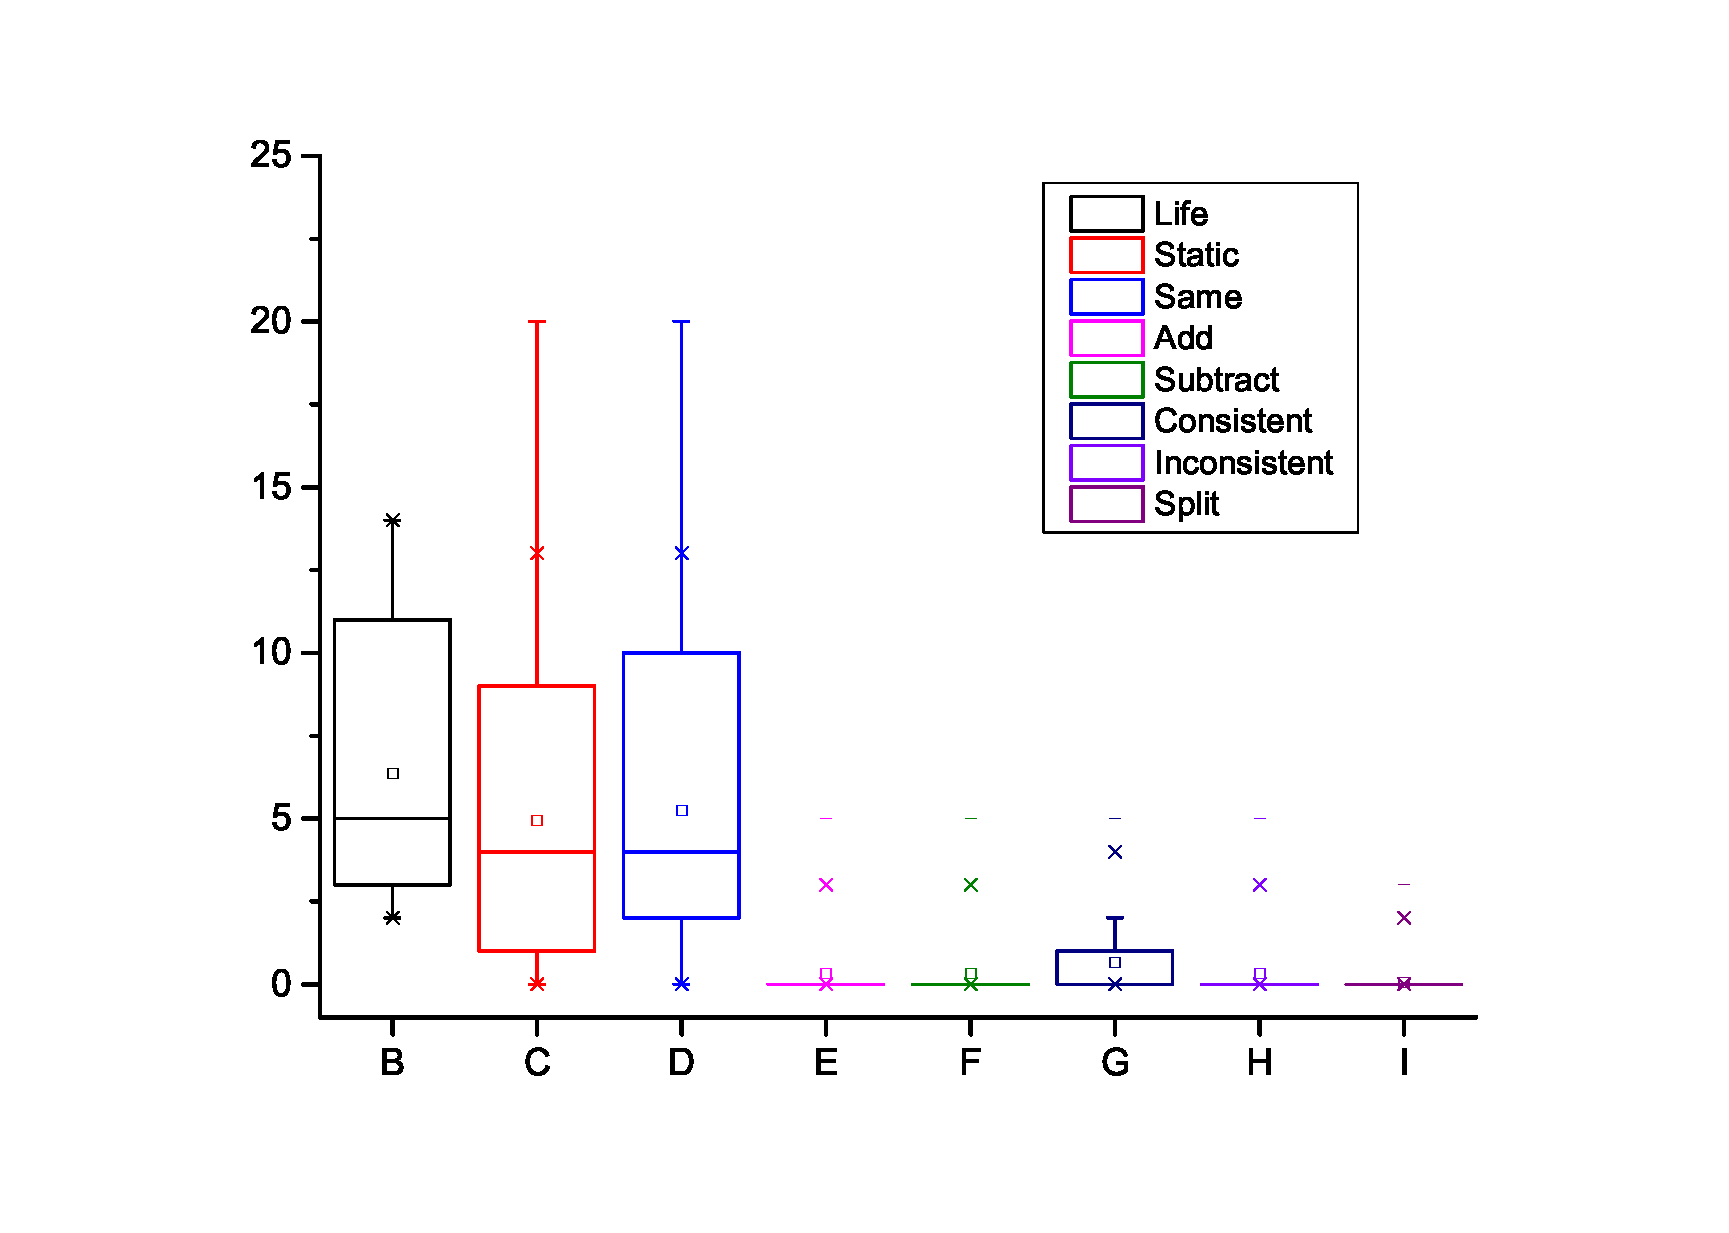
\includegraphics[width=0.4\textwidth]{Fig2-3a.eps}}}
\subfigure{\label{cgestas2}}\addtocounter{subfigure}{-2}
\subfigure[jEdit]{\subfigure[jEdit]{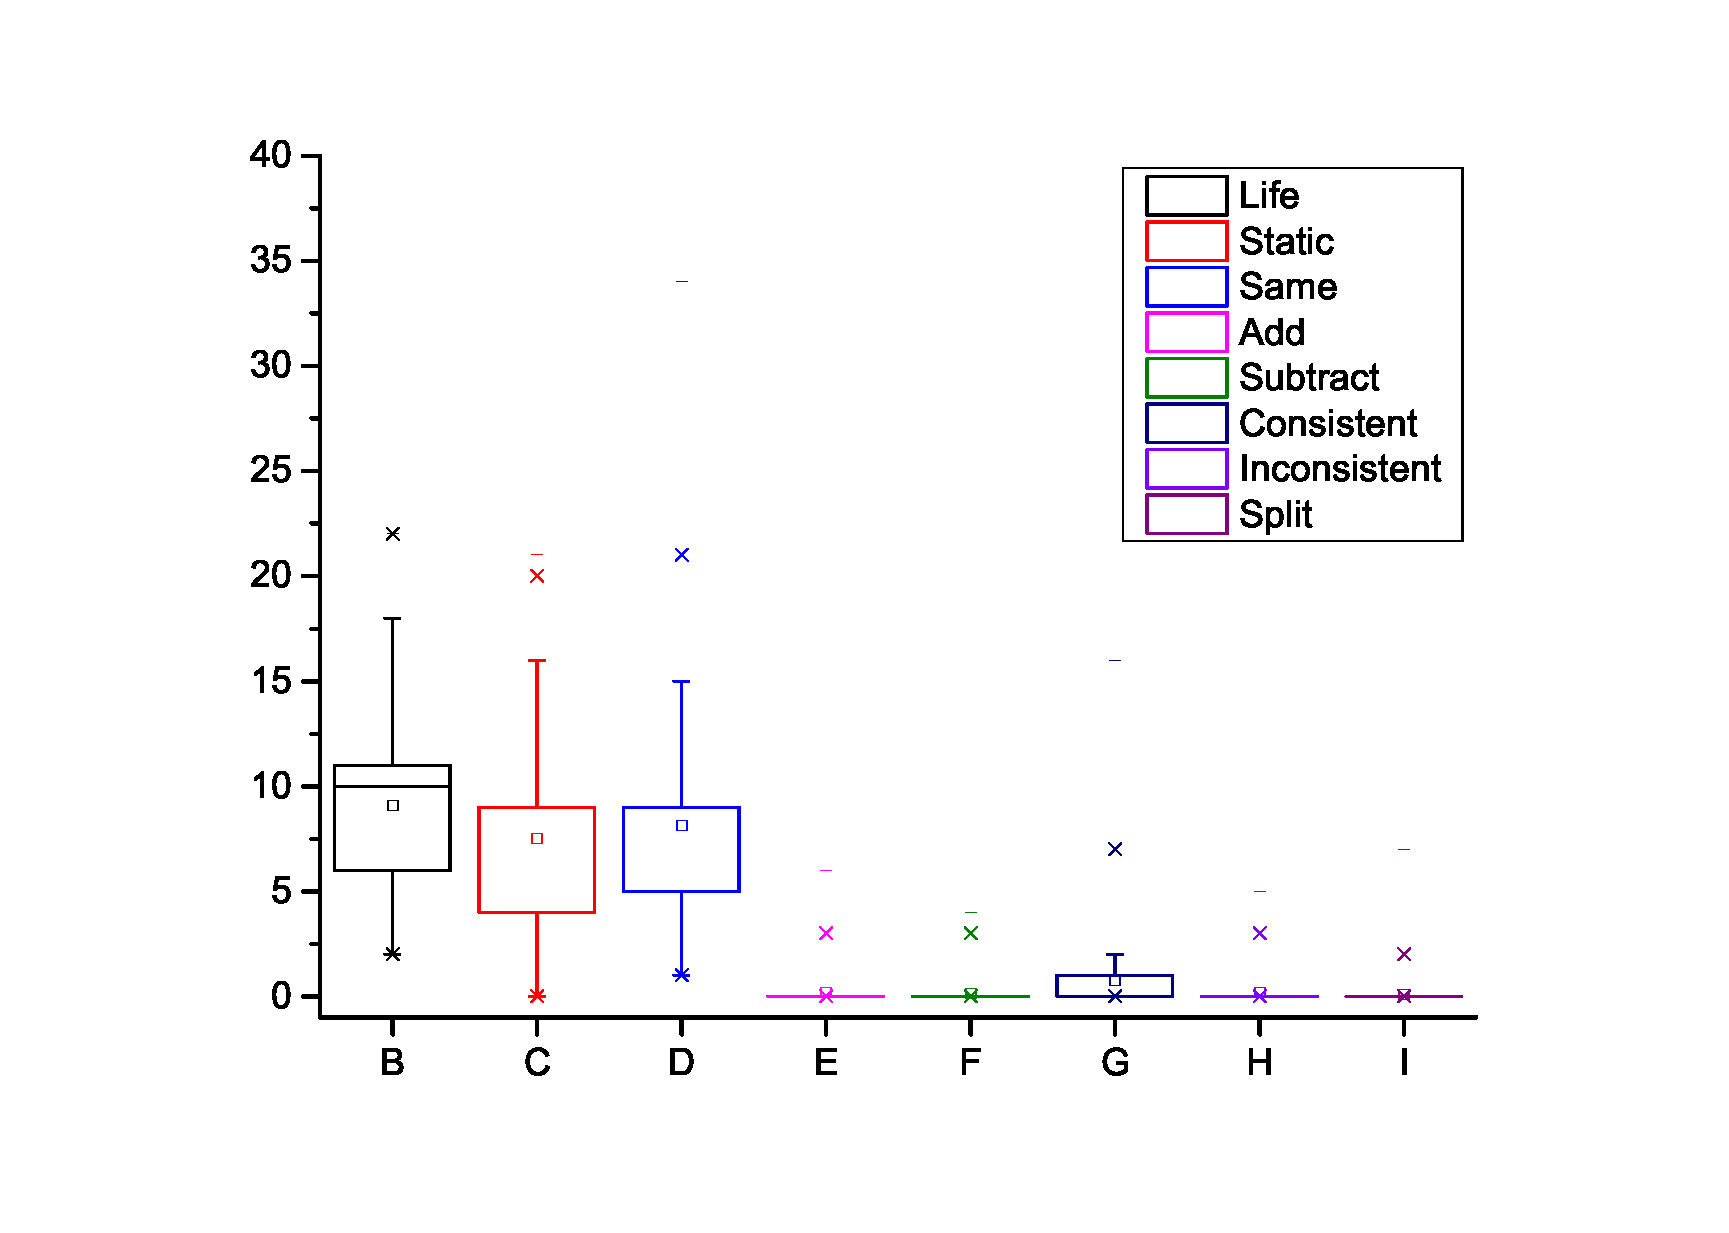
\includegraphics[width=0.4\textwidth]{Fig2-3b.eps}}}
\bicaption[cgestas]{}{克隆家系统计分析结果}{Fig.$\!$}{Clone Genealogy Statistics Results}\vspace{-1em}
\end{figure}

我们首先计算所有克隆谱系中的每个度量(包括谱系生活和克隆模式)的统计。结果绘制在图\ref{},使用“框和须”图。 第一个(最左侧)框显示关于家谱生活的统计。 对于图中的其余框,它们中的每一个代表每个克隆模式的统计。
 
我们可以看到克隆系谱在系统中存在相当长的一段时间(即{\em mean value of life}。是{\em  ArgoUML}在整个14个版本中的5个版本,以及10个版本的{\em jEdit }与整个22版本),并且只有一小部分克隆系谱存在极短(少于3版本)或极长(多于10版本)的生活。我们还看到{\em stable clone pattern}的数量远远高于{\em dynamic clone pattern}的数量。 对于{\em dynamic clone pattern},它们的数量非常少,期望{\em consistent change pattern}。{\em 这意味着克隆系谱在克隆进化的生命期间是非常稳定的。}特别地,“一致的变化”的数量超过“不一致的变化”的数量。 这意味着{\em 值得注意确定克隆更改是否应该传播到同一克隆组中的其他克隆}。
  
\begin{table}[htbp]
\bicaption[cggcluargouml]{}{ArgoUML中克隆家系的聚类结果}{Table$\!$}{Clone Genealogy Clustering Results of ArgoUML}
\vspace{0.5em}\centering\wuhao
\begin{tabular}{ccccccccccc}
\toprule[1.5pt]
 &Death&&Genealogy Life&	Static&	Same&	Add	&Subtract&	Consistent&	Inconsistent&	Split\\ 
\midrule[1pt]
Cluster0&\multirow{3}{*}{5}&Mean	&11.85366	&9.79268	&10.45122	&2.23171&	2.23171&	3.06098&	2.29268&	0.39024\\ \cline{3-11}
82&&Standard Deviation	&1.81979	&2.98861&	3.04758&	1.04585&	1.08068	&0.85125&1.07138&	0.84263\\ \cline{3-11}
(8\%)&&Median	&11&	10&	10&	2&	2&	3&	2	&0\\ \hline
Cluster1&\multirow{3}{*}{39}&Mean	&10.19221	&8.83117	&9.0961	&0.17143	&0.12208	&0.44416	&0.12208	&0.00519\\ \cline{3-11}
385&&Standard Deviation&	1.67998	&1.67552	&1.70282	&0.39754&	0.3278	&0.64761&	0.3278	&0.10193\\ \cline{3-11}
(37\%)&&Median	&11	&9	&10	&0&	0&	0&	0	&0\\ \hline
Cluster2&\multirow{3}{*}{188}&Mean	&3.29412	&1.2549	&2	&0.47059	&0.46078	&1.2598	&0.46078	&0.0098\\ \cline{3-11}
204&&Standard Deviation	&1.22847	&1.35506	&1.32427	&0.63875	&0.63822	&0.43961	&0.63822	&0.14003\\ \cline{3-11}
(20\%)&&Median	&3&	1&	2&	0&	0&	1&	0&	0\\ \hline
Cluster3&\multirow{3}{*}{348}&Mean	&2.79452	&1.79452	&1.79452	&0	&0	&0	&0	&0\\ \cline{3-11}
365&&Standard Deviation	&1.0813	&1.0813	&1.0813	&0	&0	&0	&0	&0\\ \cline{3-11}
(35\%)&&Median	&3	&2	&2	&0	&0	&0&	0&	0\\ \hline
All&\multirow{3}{*}{579}&Mean	&6.35907	&4.93629	&5.23359	&0.33301	&0.31274	&0.65541	&0.31757	&0.03475\\ \cline{3-11}
1036&&Standard Deviation	&4.02533	&4.0219	&4.06154	&0.74995	&0.74514	&0.97405	&0.75663	&0.27231\\ \cline{3-11}
(100\%)&&Median&	5&	4&	4&	0&	0&	0&	0&	0\\ \hline
\bottomrule[1.5pt]
\end{tabular}
\end{table}

\begin{table}[htbp]
\bicaption[cggclujedit]{}{jEdit中克隆家系的聚类结果}{Table$\!$}{Clone Genealogy Clustering Results of jEdit}
\vspace{0.5em}\centering\wuhao
\begin{tabular}{ccccccccccc}
\toprule[1.5pt]
&Death&&Genealogy Life&	Static&	Same&	Add	&Subtract&	Consistent&	Inconsistent&	Split\\
\midrule[1pt]
Cluster0&\multirow{3}{*}{3}&Mean	&19	&15.8	&19.2	&3	&2.3&	6	&2.7&	1.1\\ \cline{3-11}
10&&Standard Deviation	&4.83046	&4.56557&	6.42564	&1.33333&	0.94868&	4.57044&	1.41814	&2.23358\\ \cline{3-11}
(4\%)&&Median	&22&	17&	19&	3&	2	&4.5	&2.5&	0\\ \hline
Cluster1&\multirow{3}{*}{35}&Mean	&10.95205&	9.44521&	9.93836&	0.07534	&0.07534	&0.58904&	0.08219&	0.0411\\ \cline{3-11}
146&&Standard Deviation&2.35572	&2.16566&2.35832	&0.26485	&0.31262&	1.07428&	0.34254&	0.28471\\ \cline{3-11}
(62\%)&&Median&	10&	9&	9	&0&	0	&0	&0&	0\\ \hline
Cluster2&\multirow{3}{*}{24}&Mean	&6.57143&	4.75&	5.60714&	0.07143&	0.07143&	0.85714&	0.07143&	0.07143\\ \cline{3-11}
28&&Standard Deviation	&1.16837&	1.14261	&1.22744	&0.26227&0.26227	&0.97046	&0.26227	&0.37796\\ \cline{3-11}
(12\%)&&Median	&7	&5	&6&	0	&0	&1&	0&	0\\ \hline
Cluster3&\multirow{3}{*}{48}&Mean	&3.33962&	2.13208&	2.30189&	0.03774&	0	&0.20755&	0	&0\\ \cline{3-11}
53&&Standard Deviation&	0.73231	&0.92065	&0.72284&	0.19238&	0&	0.45398	&0	&0\\ \cline{3-11}
(22\%)&&Median	&3&	2&	2	&0&	0&	0	&0&	0\\ \hline
All&\multirow{3}{*}{110}&Mean	&9.07173	&7.52321&	8.1097	&0.18987&	0.1519&	0.76371	&0.173&	0.08017\\ \cline{3-11}
237&&Standard Deviation	&4.36559&	4.07926	&4.56922	&0.6903&	0.55438&	1.70588	&0.66354	&0.55033\\ \cline{3-11}
(100\%)&&Median	&10	&9	&9	&0	&0	&0	&0	&0\\ \hline
\bottomrule[1.5pt]
\end{tabular}
\end{table}

我们使用X-means聚类从{\em life}和{\em 克隆模式}之间的克隆系谱中挖掘更多信息。在表~\ref{}和~\ref{}中,我们定义了一个称为{\em Death}的特殊变量,其报告在达到实验收集的最后版本之前已经结束生命的克隆系谱的数量。通过知道一个家谱有助于{\em Death}中的计数,我们知道我们在克隆系谱实验中获得的数据是“完整的”。家谱不会被我们选择的软件版本过早地终止。因此,这些表中的第二列显示了死亡克隆系谱的编号。

根据聚类结果,所有克隆系谱可以聚类成四个聚类,如表所示。%从图。 3 /表10 \和11,
很明显{\em 在家谱生活和稳定模式之间存在强正相关}。我们非正式地定义一个家谱是{\em stable},如果它具有高百分比的{\em 稳定克隆模式},(由大量的“静态”和“相同”度量表示)。否则,我们说系谱是{\em dynamic},(也就是说,它有一个相对较大的“add”,“subtract”,“ split‘’克隆模式)。从表中,我们可以看到:{\em 大多数克隆系谱是稳定的(簇1,2,3)}。另一方面,动态系谱学少得多(在群集0中,具有长寿命,并且大多数系统中仍然存活)。它告诉我们{\em 动态克隆模式 - 特别是一致和不一致的变化 - 通常发生在更长寿的克隆系谱中。此外,动态系谱的数量很小}。这表明开发人员应该对{\em 动态系谱}采取一些措施,因为不一致的更改可能导致软件缺陷。对于簇3(表10,11中),相应的克隆系谱具有相对较短的寿命,并且它们中的大多数已经死亡。这些克隆系谱非常稳定,因为不存在不一致的模式。 {\em 因此,可以得出结论,短寿命克隆系谱中的克隆比较老的克隆更稳定。它可以给我们一个提示,开发人员可能不需要保持他们的眼睛在新创建(较短的生命)克隆系谱。但是,当他们与软件一起发展时,他们应该注意他们。}

总之,克隆系谱在整个进化中大多是稳定的。较短寿命的家谱特别稳定。 {\em 动态变化模式}通常发生在较长寿命的家谱中,即使外观依然稀少。其中,一致的变化比不一致的变化更频繁。因此,我们建议开发人员应该注意更长寿的克隆系谱,并考虑当一个克隆片段即将发生变化时允许克隆组一致变化的可能性。
 
 \BiSection{讨论和分析}{Discussion}
 
 我们的方法取决于NiCad和克隆映射算法构建克隆系谱。 我们使用NiCad检测克隆,其结果然后用于映射克隆,以便构建克隆系谱。更精细的克隆检测工具和更精确的克隆映射算法可能提高后续阶段的质量。请注意,我们的方法很大程度上取决于克隆度量的可用性。我们使用一组指标来表示克隆片段,克隆组,克隆系谱。虽然这些指标对我们有很好的影响,但我们希望将来扩展指标的收集,因为新的有趣指标可以暗示克隆与其进化之间可能存在的新关系。

在将来,我们还可以对具有更多克隆度量的不同软件进行更多的实验。我们相信,我们提出了一些更有意义的结论,以帮助克隆分析和克隆维护。我们还可以对克隆特征进行一些进一步的工作。我们认为克隆特征应该在系统维护期间的克隆分析中使用。例如,我们可以从软件中识别一些特殊的克隆,并且我们打算将其链接到克隆有害性。

 \BiSection{结论}{Conclusion}
 
在本文中,我们提出了一种通过机器学习方法从克隆及其进化中分析克隆进化特征的方法。具体来说,我们通过考虑克隆实体的生命时间证明了克隆实体的聚类(通过X平均算法)的有用性。我们的论文的贡献包括:(1)我们提出一个框架来分析克隆特征的多版本软件。 (2)我们提取一类相关的克隆度量来表征克隆片段,克隆组和克隆系谱。我们提供了关于克隆进化的三个不同的观点,从而可以从克隆进化的所有方面得出结论,从个体克隆的角度到全球的系谱观点。 (3)我们对两个软件进行了一个案例研究:{\em  ArgoUML}和{\em jEdit}来研究克隆进化特征。我们的案例研究表明克隆通常在其进化过程中非常稳定,并且克隆通常在进化的婴儿期不经历改变。因此,开发人员应该更多地关注在几次进化(也就是更长寿的克隆系谱)后存在于谱系中的(更成熟的)克隆。我们还建议开发人员应考虑在其中一个组成的克隆片段发生变化时,在整个克隆组中进行一致性更改的可能性。

我们相信这些特性可以帮助开发人员更好地理解克隆,还可以提供一些指导来维护和管理软件开发中的克隆。在未来,我们打算通过纳入更多的度量来改进我们对克隆组和克隆基因生态学的分析。关于克隆组和谱系关系的结论可以被看作是克隆进化的特征。这些功能可能有助于克隆管理。